\documentclass{gescons}

\genre {Entrevista}
\author{Luimara Schmit}
\title{Mutatis Mutandis: Teoria e~Prática da Reciclagem Existencial}
\paginaurl{https://www.youtube.com/live/FXWtZpHxP8k}

\begin{document}
    \makeentrevistatitle
    \coverart{back/Luimara_Schmit}

    \begin{multicols}{2}

\begin{center}
    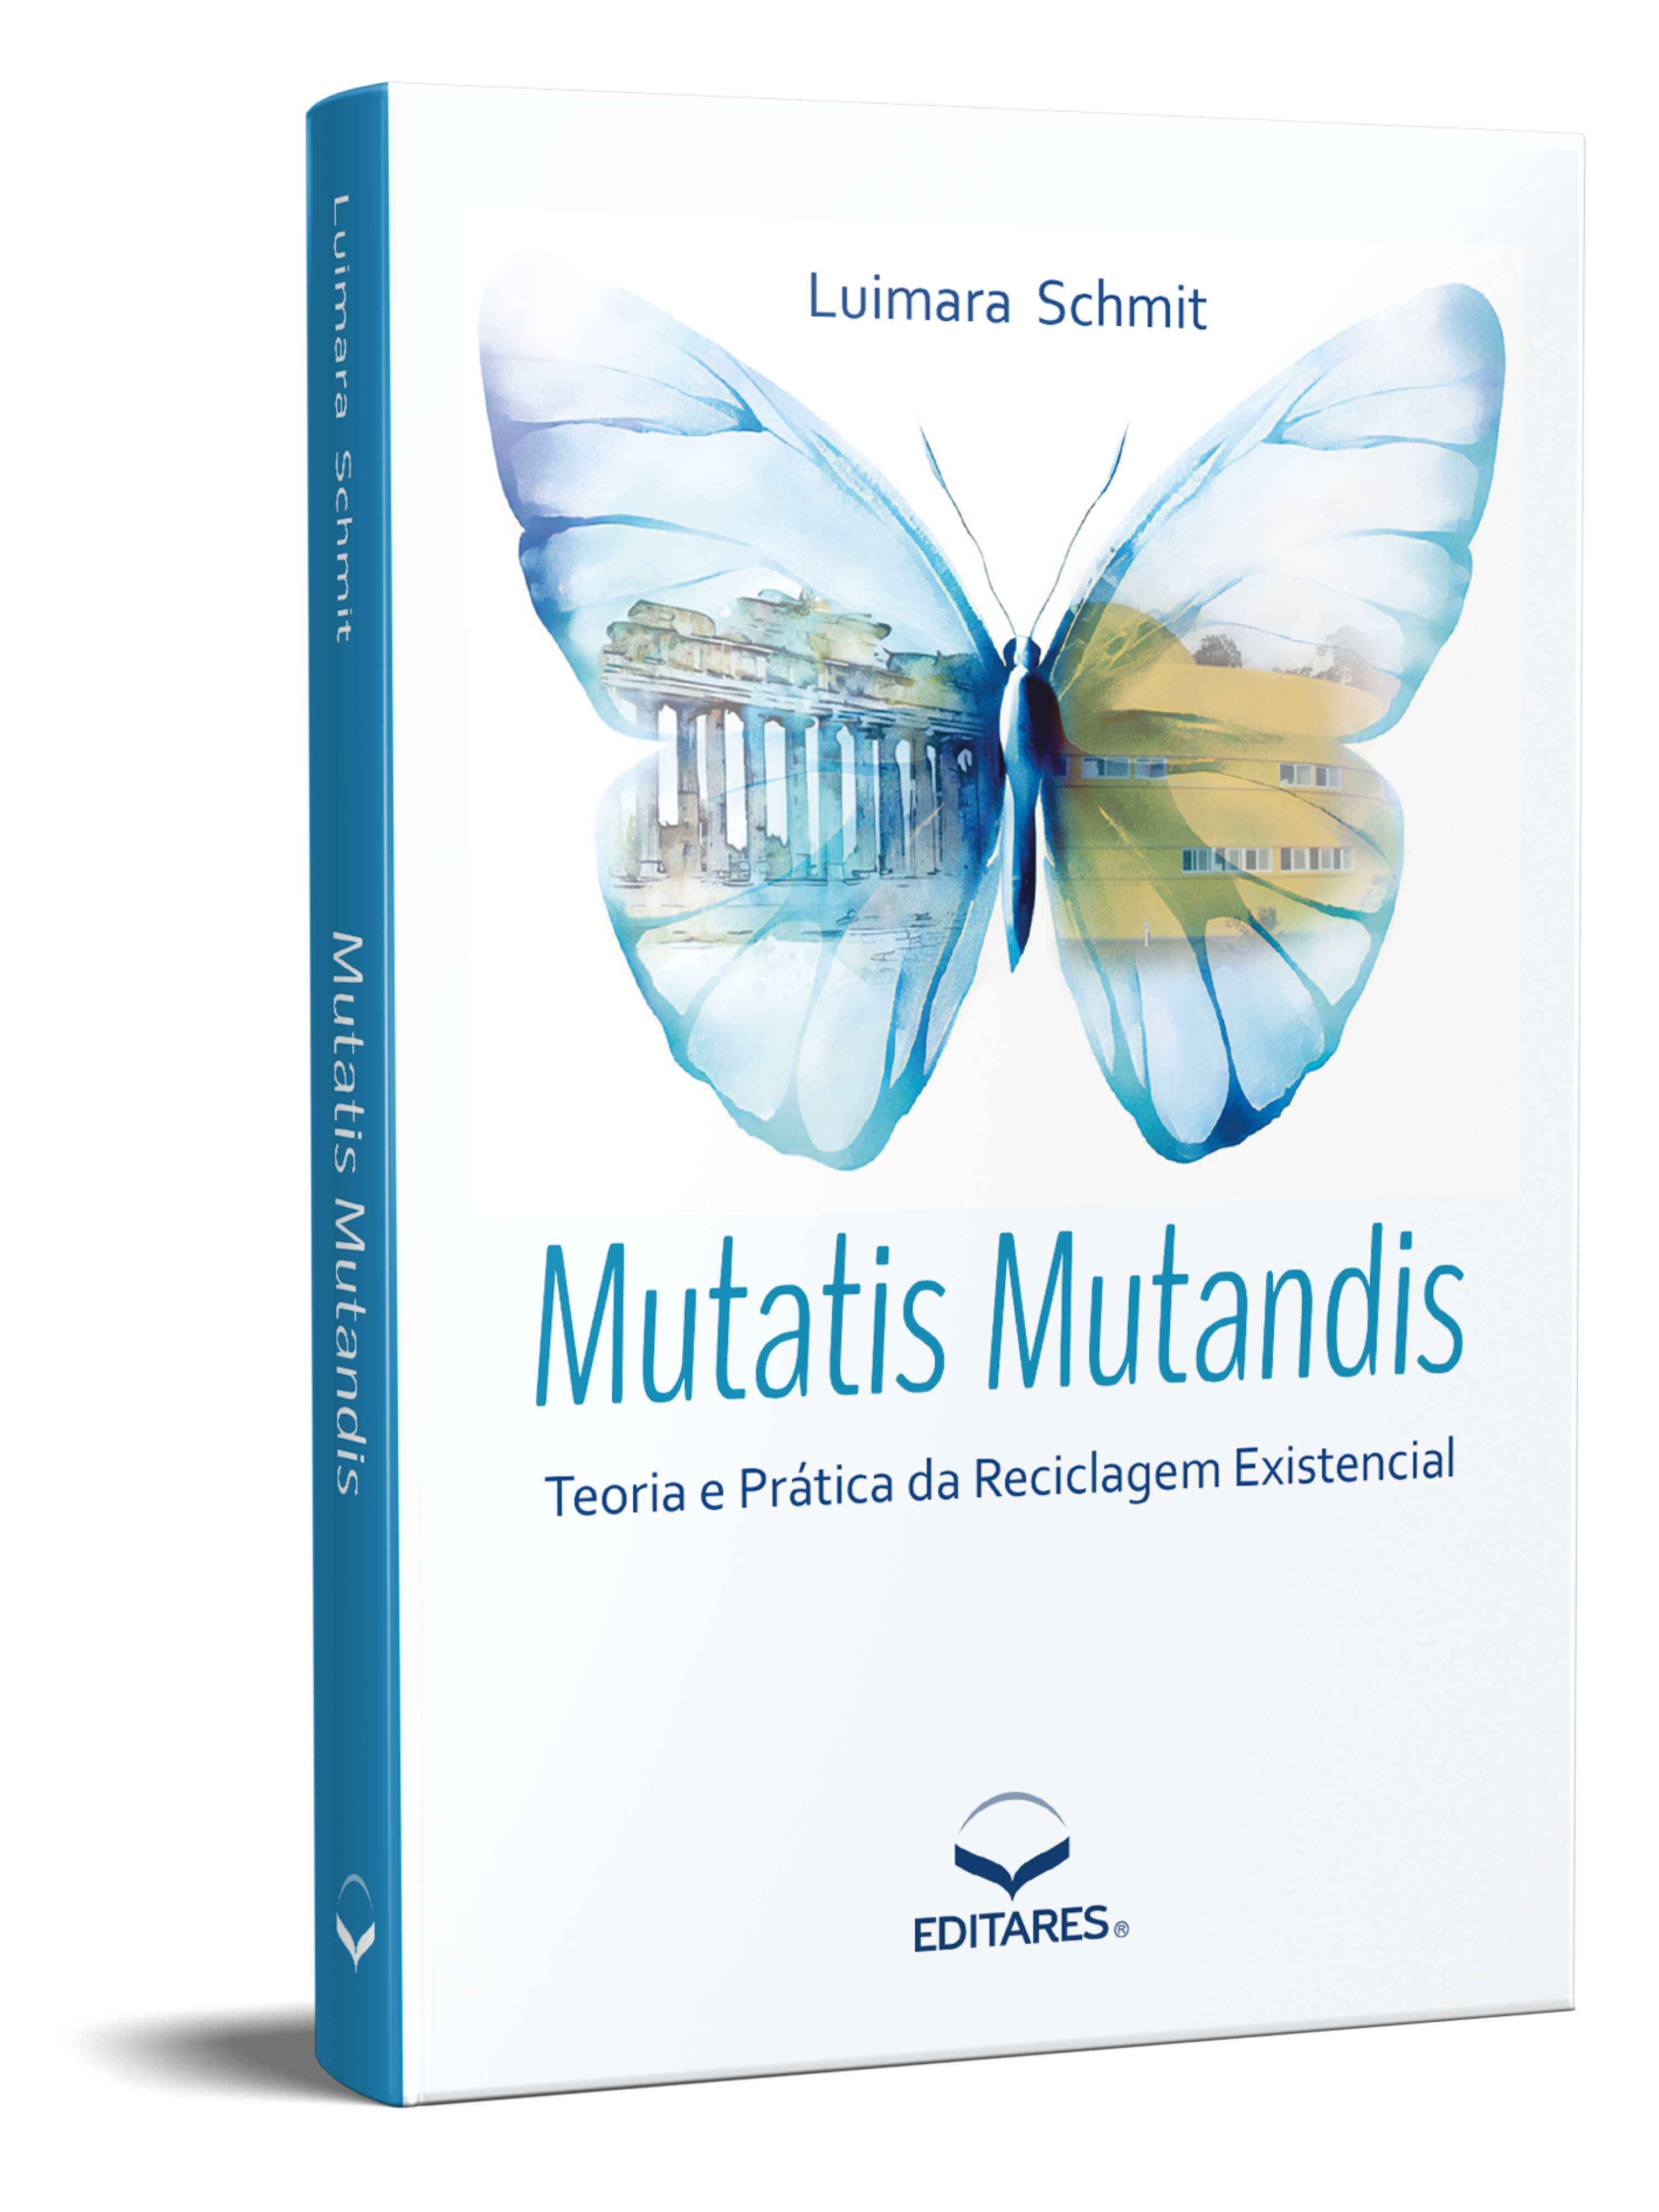
\includegraphics[width=6cm]{articles/entrevista/mockups/Luimara}
\end{center}

\textbf{1. Qual foi a~motivação para a~escrita da obra? Por que a~definição deste tema para publicação de um livro?}


O tema principal do livro é~a~\emph{reciclagem existencial,} técnica conscienciológica que objetiva a~mudança para melhor dos aspectos da vida humana e~interdimensional para quem estiver predisposto a~adotar novo conjunto de valores pró-evolutivos.

A primeira seção, composta por perguntas e~respostas, propicia a~ampliação do conhecimento teórico sobre recéxis, enquanto a~segunda seção oportuniza a~autopesquisa prática, contendo 100 perguntas para a~recexometria mais ampla. Para o~autodiagnóstico mais assertivo é~apresentado o~\emph{Recexograma,} no formato de planilha. Assim, os interessados têm a~possibilidade de aprofundar a~compreensão do tema e~se instrumentalizarem para a~aplicação didática da recéxis.

Identifico que o~gosto pela leitura e~a~afinidade com a~escrita são inatos. Reconheço que o~incentivo e~o~exemplarismo do professor Waldo Vieria, associados à~compreensão do potencial interassistencial e~de autorrevezamento multiexistencial de uma gescon, foram os propulsores para as autorrenovações essenciais à~dedicação para a~escrita do livro.

A escolha do tema relacionado à~\emph{reciclagem existencial} tem relação com as vivências e~as necessidades pessoais identificadas enquanto intermissivista, conscienciômetra e~aplicante da \emph{técnica da recéxis} há mais de duas décadas.

Tendo em vista que não dispunha de instrumento específico, elaborei o~\emph{Programa de Recéxis,} incluindo o~\emph{Recexograma} (composto por 100 itens para auxiliar no acompanhamento da performance pessoal nas diversas áreas da vida) e~o~\emph{Plano de Ação Recexométrico.} Desse modo, a~partir do programa de autorrenovações continuadas, pautado na proposta de reciclagem prazerosa, possibilita-se a~conquista do autoequilíbrio holossomático, alinhado aos objetivos de alcançar a~desperticidade e~o~completismo existencial.

\textbf{2. Quais foram as principais percepções, intra e~extrafísicas, durante a~pesquisa e~a~escrita da obra?}

Percebi a~diversificação e~o~aumento de demandas assistenciais familiares, profissionais e~no voluntariado, sinalizando a~checagem da sustentabilidade pessoal afim aos temas pesquisados. Do ponto de vista multidimensional, observei a~sutilização do parapsiquismo, o~crescendo gradual das parapercepções e~a~ampliação da captação de inspirações, a~partir da maior conexão com o~amparador de função. O~título principal, \emph{Mutatis Mutandis,} foi inspirado extrafisicamente na tenepes e~complementou de modo instigante a~abordagem teática à~recéxis.

\textbf{3. Qual o~maior aprendizado com a~escrita desta obra?}

O aumento da \emph{autoconscientização multidimensional,} incluindo inusitado rol de sincronicidades, está contribuindo para a~ampliação do autorrealismo e~a~sensação de \emph{ser consciência.} Compreendi, na prática, que a~escrita conscienciológica é~teática e~requer exemplarismo. Também propicia a~qualificação de habilidades interassistenciais e~do respeito interconsciencial, pois cada qual estabelece o~ritmo e~o~limite para as autorreciclagens.

\textbf{4. O~que poderia dizer como incentivo para que mais pesquisadores invistam na publicação de obras conscienciológicas?}

Compartilhe suas experiências!

Elaborar \emph{gestação consciencial} sob a~perspectiva do neoparadigma é~desafiador e~gratificante. O~livro é~um \emph{investimento evolutivo} muito significativo e~pode oportunizar a~catalisação de recomposições grupocármicas insuspeitas.

% \begin{pullquote}
% ``Elaborar gestação consciencial sob a~perspectiva do neoparadigma é~desafiador e~gratificante.''
% \end{pullquote}
% 
    
    \end{multicols}
\end{document}



